%
% File: chap01.tex
%
\let\textcircled=\pgftextcircled
\chapter{Reactor Heat Generation}
\label{chap:intro}

\initial{S}everal exercises from the book written by M. M. El Wakil~\cite{book01} are tackled in this homework. The problems in this section relate to the seventh and eigth chapter of the book, covering the subject of heat conduction in reactor elements.

%=======
\section{[7-6] - Rectangular fin}
\label{prob71}

\subsection{Problem}
\textit{A very long fin is rectangular in cross-section $0.48 * 0.24$ in. It generates \num{2e6} $Btu.h^{-1}.ft^{-3}$. The fin base is at $1000{}^\circ F$. It is cooled by a gas at $600{}^\circ F$ with a uniform heat transfer coefficient $100\ Btu.h^{-1}.ft^{-2}.{}^\circ F^{-1}$. Using a network with $\Delta x = 0.12$ in., write the necessary set of finite difference equations for the nodal points and solve by any one of the techniques at your command. $k$ for the fin material $= 10\ Btu.h^{-1}.ft^{-1}.{}^\circ F^{-1}$}

\subsection{Solution}

First, one can note that the problem is missing a graph. The considered geometry is given in Figure~\ref{fig71}.

\begin{figure}[H]
\centering
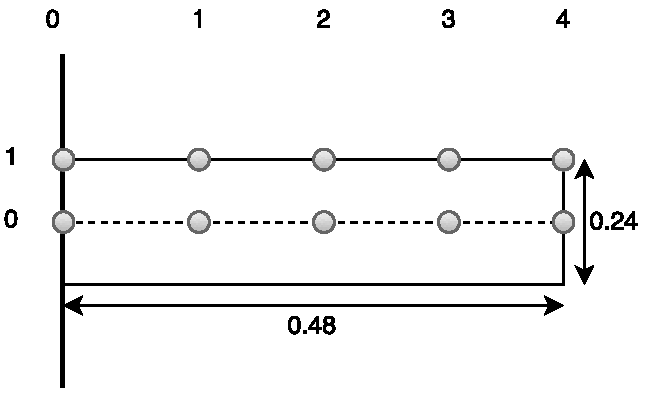
\includegraphics[scale=1]{fig/schema.pdf}
\caption{Representation of the problem geometry}
\label{fig71}
\end{figure}

We can identify four types of nodes: inner, y-bound (next to the upper boundary), x-bound (next to the right boundary) and corner.

The inner node temperature $T_n$ is given by Equation~\ref{eq71}.

\begin{equation}\label{eq71}
T_n = \frac{T_{n-\Delta x} + T_{n+\Delta x} + T_{n-\Delta y} + T_{n+\Delta y}}{4} + \frac{\Delta T_g}{2}
\end{equation}

In our case, we can see that $T_{n-\Delta y} = T_{n+\Delta y}$ by symmetry for the inner nodes. Consequently, we obtain Equation~\ref{eq72}.

\begin{equation}\label{eq72}
T_n = \frac{T_{n-\Delta x} + T_{n+\Delta x} + 2T_{n+\Delta y}}{4} + \frac{\Delta T_g}{2}
\end{equation}

For the x-bound nodes, we can write Equation~\ref{eq73}.


\begin{equation}\label{eq73}
T_n = \frac{T_{n-\Delta x} + T_{n+\Delta y} + Bi_{\Delta x}T_f}{2 + 2Bi_{\Delta x}} + \frac{\Delta T_g}{2+Bi_{\Delta x}}
\end{equation}

For the y-bound nodes, we can write Equation~\ref{eq74}

\begin{equation}\label{eq74}
T_n = \frac{T_{n-\Delta x} + T_{n+\Delta x} + 2T_{n+\Delta y} + 2Bi_{\Delta x}T_f}{4 + 2Bi_{\Delta x}} + \frac{\Delta T_g}{2+Bi_{\Delta x}}
\end{equation}

And finally, for the corner node, we can write (as seen in problem 7.1 previously) Equation~\ref{eq75}.

\begin{equation}\label{eq75}
T_n = \frac{T_{n-\Delta x} + T_{n+\Delta y} + 2Bi_{\Delta x}T_f}{2 + 2Bi_{\Delta x}} + \frac{\Delta T_g}{2+2Bi_{\Delta x}}
\end{equation}

A few exceptions can be noted. Indeed, the two leftmost points, on the base of the fin, are given to be at $1000{}^\circ F$.

We can consequently write the matrix $A$. 


\setcounter{MaxMatrixCols}{30}
\tiny
\[
A =
  \begin{bmatrix}
1     & 0    & 0     & 0     & 0     & 0     & 0     & 0     & 0     & 0          \\
0     & 1    & 0     & 0     & 0     & 0     & 0     & 0     & 0     & 0          \\
-0.25 & 0    & 1     & -0.5  & -0.25 & 0     & 0     & 0     & 0     & 0          \\
0     & \frac{-1}{2Bi_{\Delta x}+4}     & \frac{-1}{Bi_{\Delta x}+2} & 1 & 0     & \frac{-1}{2Bi_{\Delta x}+4}  & 0 & 0     & 0     & 0          \\
0 & 0 & -0.25 & 0    & 1     & -0.5  & -0.25 & 0     & 0     & 0           \\
0 & 0 & 0     & \frac{-1}{2Bi_{\Delta x}+4}     & \frac{-1}{Bi_{\Delta x}+2} & 1 & 0     & \frac{-1}{2Bi_{\Delta x}+4}  & 0 & 0           \\
0 & 0 & 0 & 0 & -0.25 & 0    & 1     & -0.5  & -0.25 & 0            \\
0 & 0 & 0 & 0 & 0     & \frac{-1}{2Bi_{\Delta x}+4}     & \frac{-1}{Bi_{\Delta x}+2} & 1 & 0     & \frac{-1}{2Bi_{\Delta x}+4}           \\
0 & 0 & 0 & 0 & 0     & 0 & \frac{-1}{Bi_{\Delta x}+2} & 0 & 1 & \frac{-1}{Bi_{\Delta x}+2} \\
0 & 0 & 0 & 0 & 0     & 0 & 0 & \frac{-1}{2Bi_{\Delta x}+2} & \frac{-1}{2Bi_{\Delta x}+2} & 1 \\
  \end{bmatrix}
\]

\normalsize

$\frac{\Delta T_g}{2}$ can be calculated using $\Delta T_g = \frac{(\Delta x)^2 q'''}{2k}$. $T_f$, the temperature of the gas, is known. We can thus obtain $b$.
\tiny
\[
b =
  \begin{bmatrix}
1000 \\
1000 \\
7.2 \\
229.5\\
7.2\\
229.5\\
7.2 \\
229.5\\
229.5\\
330.5\\
   \end{bmatrix}
\]

\normalsize

The equation $A.x = b$ can thus be solved, using Python. The python script is given in~\ref{py1}. We obtain the following results (Equation~\ref{eq76}):

\begin{equation}\label{eq76}
\begin{aligned}
T(0,0) = 1000.0\\
T(0,1) = 1000.0\\
T(1,0) = 797.5\\
T(1,1) = 736.6\\
T(2,0) = 696.6\\
T(2,1) = 659.4\\
T(3,0) = 650.1\\
T(3,1) = 630.3\\
T(4,0) = 623.3\\
T(4,1) = 614.5\\
\end{aligned}
\end{equation}


\newpage
\subsubsection{Python script}
\label{py1}
\begin{lstlisting}[language=python]
import numpy as np

m = 10    # size of system is m x m

dx = 0.12
deltax, k, qtriple, h = (dx/12)**2, 10., 2.e6, 100.    # BG units
tb = 1000.
ts = 600.
dtg = (0.5*deltax)*qtriple/k
bi = h * dx / k

amat = np.zeros((m,m))
b = np.zeros(m)
    
amat[0,0] = 1.
amat[1,1] = 1.
b[0] = tb
b[1] = tb

for i in range(2, m, 2):
    try:
        amat[i,i-2] = -0.25
        amat[i,i] = 1.
        amat[i,i+1] = -0.5
        amat[i,i+2] = -0.25
        b[i] = dtg/2.
    except IndexError:
        break

for i in range(3, m, 2):
    try:
        amat[i,i-2] = -1/(2*bi+4)
        amat[i,i-1] = -1/(bi+2)
        amat[i,i] = 1.
        amat[i,i+2] = -1/(2*bi+4)
        b[i] = (bi*ts + dtg)/(bi+2)
    except IndexError:
        break

amat[m-1,m-1] = 1.
amat[m-1,m-2] = -1/(2*bi+2)
amat[m-1,m-3] = -1/(2*bi+2)
b[m-1] = (2*bi*ts + dtg)/(2*bi+2)


amat[m-2,m-2] = 1.
amat[m-2,m-1] = -1/(bi+2)
amat[m-2,m-4] = -1/(bi+2)
b[m-2] = (bi*ts + dtg)/(bi+2)
print(b)
ysol = np.linalg.solve(amat,b)

print('Temperature solution:')

temp = []
for i in range(5):
    for j in range(2):
        temp.append("T(%s,%s)" % (i, j))
        
for i,t in enumerate(temp):
    print("%s = %.1f" % (t, ysol[i]))
    
# check of solution: 
if not np.allclose(np.dot(amat, ysol), b):
    print("Solution does not match!")
\end{lstlisting}
\newpage

\section{[7-13] - Heat flux}
\label{prob72}

\subsection{Problem}
\textit{A long fuel element has a rectangular cross-section $1*2$ in. It generates \num{1e6} $Btu.h^{-1}.ft^{-3}$ and has a thermal conductivity of $1.085\ Btu.h^{-1}.ft^{-1}.{}^\circ F^{-1}$. All surfaces are held at $1000{}^\circ F$. Find the heat flux, $Btu.h^{-1}.ft^{-2}$ at the center point of each side using the approximate analytical solution of section 7-13.}

\subsection{Solution}

The book~\cite{book01} gives us a solution for a long rectangular fuel element (Equations 7-34 to 7-44). It is given here by Equation~\ref{eq77}.

\begin{equation}\label{eq77}
T(x,y) = \frac{3}{4}\frac{q'''}{k(a^2+b^2)}(a^2-x^2)(b^2-y^2)
\end{equation}

However, this solution is obtained for different boundary conditions ($T_s = 0{}^\circ F$). In our case, $T_s = 1000{}^\circ F$. Then, we can rewrite Equation~\ref{eq77} to Equation~\ref{eq78} to account for this different boundary condition.


\begin{equation}\label{eq78}
T(x,y) = \frac{3}{4}\frac{q'''}{k(a^2+b^2)}(a^2-x^2)(b^2-y^2) + 1000 = C(a^2-x^2)(b^2-y^2) + 1000
\end{equation}

The heat flux is given in the x-direction by Equation~\ref{eq79} and in the y-direction by Equation~\ref{eq710}.


\begin{equation}\label{eq79}
q''_x = -k\frac{\partial T}{\partial x}
\end{equation}

\begin{equation}\label{eq710}
q''_y = -k\frac{\partial T}{\partial y}
\end{equation}

Consequently, we can write Equations~\ref{eq711} and~\ref{eq712}.

\begin{equation}\label{eq711}
q''_x = -2kCx(y^2-b^2)
\end{equation}

\begin{equation}\label{eq712}
q''_y = -2kCy(x^2-a^2)
\end{equation}

At the center point of each side, we have Equations~\ref{eq713} and~\ref{eq714}.

\begin{equation}\label{eq713}
q''_x\bigg\rvert_{x=a, y=0} = 2kCab^2
\end{equation}

\begin{equation}\label{eq714}
q''_y\bigg\rvert_{x=0, y=b} = 2kCba^2
\end{equation}

So, we obtain $q''_x = \text{\num{2.5e4}}\ Btu.h^{-1}.ft^{-2}$ and $q''_y = \text{\num{5.0e4}}\ Btu.h^{-1}.ft^{-2}$.

\section{[8-1] - Cool down time}
\label{prob73}

\subsection{Problem}
\textit{A 2 in. diam. steel ball initially at a uniform $850{}^\circ F$, is suddenly subjected to an environment at $200{}^\circ F$. The natural convection heat transfer coefficient is $2\ Btu.h^{-1}.ft^{-2}.{}^\circ F^{-1}$. Find the time necessary for the ball to cool down to $300{}^\circ F$.}

\subsection{Solution}

The book~\cite{book01} gives us the relationship between the temperature in a two-bodies problem, Equation~\ref{eq715}.

\begin{equation}\label{eq715}
\frac{T_f - T(t)}{T_f - T_i} = e^{-t/\tau}
\end{equation}

Where:
\begin{conditions}
\tau & $\frac{c_1 \rho_1 V_1}{hA_1}$ \\
1 & index relative to the cooling body
\end{conditions}

Knowing that the cooling body is a steel ball, we can obtain its density and specific heat capacity. Knowing it is a sphere, we can obtain its surface area and volume. The heat transfer coefficient being known, we can thus calculate $\tau = \frac{0.12 * 490 * \frac{4\pi * (0.0833)^3}{3}}{2 * 4\pi * (0.0833)^2} = 0.816$. Consequently, we have Equation~\ref{eq716}.

\begin{equation}\label{eq716}
\frac{200 - 300}{200 - 850} = 0.154 = e^{-t/\tau}
\end{equation}

\begin{equation}\label{eq717}
t = -\tau \ln (0.154) = 1.528\ h
\end{equation}

The ball will cool down to $300{}^\circ F$ in $1.528\ h$, or roughly an hour and a half.

\section{[8-4] - Unsteady fuel element}
\label{prob74}

\subsection{Problem}
\textit{A flat-plate fuel element $1.25 * 0.25$ in. in cross section is initially at a uniform $1000{}^\circ F$. Suddenly heat was generated at the rate of \num{1.5e7} $Btu.h^{-1}.ft^{-3}$. All surfaces were maintained at $1000{}^\circ F$. Find by a numerical technique the time it takes the element to reach a maximum temperature $99.5\%$ of the way to maximum steady-state temperature. $k=1.085\ Btu.h^{-1}.ft^{-1}.{}^\circ F^{-1}$. $c = 0.06\ Btu.lb^{-1}.{}^\circ F^{-1}$. $\rho = 740 lb.ft^{-3}$.}

\subsection{Solution}

The surface temperatures staying at $T_s = 1000{}^\circ F$, and using a symmetry argument, only five temperatures are to be obtained in a mesh with $\Delta x = \Delta y = 0.125$ in. For precision, I decided to refine the mesh (the impact is minimal), using $\Delta x = 0.0625$. Those are all temperatures in the inner part of the plate.

The book~\cite{book01} tells us that in this case, the temperature at a time $t+\Delta t$ is given by Equation~\ref{eq718}.

\begin{equation}\label{eq718}
T_n^{t+\Delta t} = (1-4Fo)T_n^t + Fo(T_{n+\Delta x}^t + T_{n-\Delta x}^t + T_{n+\Delta y}^t + T_{n-\Delta y}^t) + 2Fo\Delta T_g
\end{equation}

Consequently, we can obtain the next timestep temperature for each point in our design. This system is solved using the python script given in~\ref{py2}.

The steady-state solutions are obtained using the largest possible time steps, for $Fo=0.25$. We obtain the following steady-state temperature:
\tiny
\begin{equation}\label{eq719}
\begin{aligned}
T(0,0) = 1000.0\\
T(0,1) = 1000.0\\
T(0,2) = 1000.0\\
T(1,0) = 1000.0\\
T(1,1) = 1300.8\\
T(1,2) = 1388.6\\
T(2,0) = 1000.0\\
T(2,1) = 1439.5\\
T(2,2) = 1577.7\\
T(3,0) = 1000.0\\
T(3,1) = 1504.4\\
T(3,2) = 1668.2\\
T(4,0) = 1000.0\\
T(4,1) = 1535.1\\
T(4,2) = 1711.3\\
T(5,0) = 1000.0\\
T(5,1) = 1549.5\\
T(5,2) = 1731.7\\
T(6,0) = 1000.0\\
T(6,1) = 1556.4\\
T(6,2) = 1741.3\\
T(7,0) = 1000.0\\
T(7,1) = 1559.6\\
T(7,2) = 1745.9\\
T(8,0) = 1000.0\\
T(8,1) = 1561.1\\
T(8,2) = 1748.0\\
T(9,0) = 1000.0\\
T(9,1) = 1561.7\\
T(9,2) = 1748.9\\
T(10,0) = 1000.0\\
T(10,1) = 1561.9\\
T(10,2) = 1749.2\\
\end{aligned}
\end{equation}
\normalsize
The $99.5\%$ value of the maximum temperature is thus $1740.5{}^\circ F$. By refining the time step, using $Fo=0.1$, we can see that this happens at the 74th step. This corresponds to a time of $74 * \frac{(\Delta x)^2 * 0.1}{\alpha} = \frac{\text{\num{0.0002}}}{\alpha}$. The thermal diffusivity $\alpha$ can be obtained using the relation~\ref{eq720}.

\begin{equation}\label{eq720}
\alpha = \frac{k}{\rho c}
\end{equation}

We obtain $\alpha = 0.024\ ft^{2}.h^{-1}$. This gives us a time $t = 0.0084\ h = 30 \ s$ necessary to reach $99.5\%$ of the maximum steady temperature.

\newpage
\subsubsection{Python script}
\label{py2}
\begin{lstlisting}[language=python]
# initialize temp. values
t11, t21, t31, t41, t51, t61, t71, t81, t91, t101 = 1000., 1000., 1000., 1000., 1000., 1000., 1000., 1000., 1000., 1000.
t12, t22, t32, t42, t52, t62, t72, t82, t92, t102 = 1000., 1000., 1000., 1000., 1000., 1000., 1000., 1000., 1000., 1000.
dx = 0.125/2
deltax, k, qtriple = (dx/12)**2, 1.085, 1.5e7    # BG units
ts = 1000.
dtg2 = (0.5*deltax)*qtriple/(k)
fo=0.25
print('temperature solution (degrees F):')
# iterate:
for i in range(51):
    t11n = (1-4*fo)*t11+fo*(t21+2*ts+t12) + 2*fo*dtg2
    t21n = (1-4*fo)*t21+fo*(t31+t11+t22+ts) + 2*fo*dtg2
    t31n = (1-4*fo)*t31+fo*(t41+t21+t32+ts) + 2*fo*dtg2
    t41n = (1-4*fo)*t41+fo*(t51+t31+t42+ts) + 2*fo*dtg2
    t51n = (1-4*fo)*t51+fo*(t61+t41+t52+ts) + 2*fo*dtg2
    t61n = (1-4*fo)*t61+fo*(t71+t51+t62+ts) + 2*fo*dtg2
    t71n = (1-4*fo)*t71+fo*(t81+t61+t72+ts) + 2*fo*dtg2
    t81n = (1-4*fo)*t81+fo*(t91+t71+t82+ts) + 2*fo*dtg2
    t91n = (1-4*fo)*t91+fo*(t101+t81+t92+ts) + 2*fo*dtg2
    t101n = (1-4*fo)*t101+fo*(2*t91+ts+t102) + 2*fo*dtg2

    t12n = (1-4*fo)*t12+fo*(2*t11+ts+t22) + 2*fo*dtg2
    t22n = (1-4*fo)*t22+fo*(t12+t32+2*t21) + 2*fo*dtg2
    t32n = (1-4*fo)*t32+fo*(t22+t42+2*t31) + 2*fo*dtg2
    t42n = (1-4*fo)*t42+fo*(t32+t52+2*t41) + 2*fo*dtg2
    t52n = (1-4*fo)*t52+fo*(t42+t62+2*t51) + 2*fo*dtg2
    t62n = (1-4*fo)*t62+fo*(t52+t72+2*t61) + 2*fo*dtg2
    t72n = (1-4*fo)*t72+fo*(t62+t82+2*t71) + 2*fo*dtg2
    t82n = (1-4*fo)*t82+fo*(t72+t92+2*t81) + 2*fo*dtg2
    t92n = (1-4*fo)*t92+fo*(t82+t102+2*t91) + 2*fo*dtg2
    t102n = (1-4*fo)*t102+fo*(2*t92+2*t101) + 2*fo*dtg2
    # roll values
    t11, t21, t31, t41, t51, t61, t71, t81, t91, t101 = t11n, t21n, t31n, t41n, t51n, t61n, t71n, t81n, t91n, t101n
    t12, t22, t32, t42, t52, t62, t72, t82, t92, t102 = t12n, t22n, t32n, t42n, t52n, t62n, t72n, t82n, t92n, t102n
    if i % 5 == 0:
        print('number of time steps: ', i+1)
        print(t12, t22, t32, t42, t52, t62, t72, t82, t92, t102)
\end{lstlisting}
\newpage

\section{[H1] - Trigonomy solution}
\label{prob75}

\subsection{Problem}
\textit{Let $T(x,y) = C \cos \left(\frac{\pi}{2a}x \right) \cos \left(\frac{\pi}{2b}y \right)$ and consider the steady-state heat conduction problem (7-34) and (7-35) of the textbook. (a) By using the approximate analytic method of section 7-13, complete the solution for the coefficient $C$ that was begun in class. (b) Let $a = b$ so that the domain becomes a square. With $x$ and $y$ in terms of $a$, and $T$ in units of $\frac{q'''a^2}{k}$, generate (i) a surface plot of the approximate solution, and (ii) a contour plot of the approximate solution. You may use software of your choice, whether it is Mathematica, Matlab, Python, or other.}

\subsection{Solution}

We assume a solution of the form $T(x,y) = C \cos \left(\frac{\pi}{2a}x \right) \cos \left(\frac{\pi}{2b}y \right)$. This solution verifies Equation~\ref{eq721}.

\begin{equation}\label{eq721}
\int_0^b \frac{\partial T}{\partial x}\bigg\rvert_{x=a} dy + \int_0^a \frac{\partial T}{\partial y}\bigg\rvert_{y=b} dx + \frac{q'''ab}{k} = 0
\end{equation}

We can solve the partial differential first.

\begin{equation}\label{eq722}
\frac{\partial T}{\partial x}\bigg\rvert_{x=a} = -C \frac{\pi}{2a} \sin \left(\frac{\pi}{2a}x \right) \cos \left(\frac{\pi}{2b}y \right) \bigg\rvert_{x=a} = -C \frac{\pi}{2a}\cos \left(\frac{\pi}{2b}y \right)
\end{equation}


\begin{equation}\label{eq723}
\frac{\partial T}{\partial x}\bigg\rvert_{x=a} = -C \frac{\pi}{2b}\cos \left(\frac{\pi}{2a}x \right)
\end{equation}

Integrating, we obtain:

\begin{equation}\label{eq724}
\int_0^b \frac{\partial T}{\partial x}\bigg\rvert_{x=a} dy = -C \int_0^b \frac{\pi}{2a}\cos \left(\frac{\pi}{2b}y \right) dy
\end{equation}

\begin{equation}\label{eq725}
\int_0^b \frac{\partial T}{\partial x}\bigg\rvert_{x=a} dy = -C \frac{b}{a}
\end{equation}


\begin{equation}\label{eq726}
\int_0^a \frac{\partial T}{\partial y}\bigg\rvert_{y=b} dx = -C \frac{a}{b}
\end{equation}

Consequently, replacing in Equation~\ref{eq721} and reorganizing:


\begin{equation}\label{eq726}
C = \frac{q'''(ab)^2}{k(a^2 + b^2)}
\end{equation}

If $a = b$, then we have $C = \frac{q'''a^2}{2k}$.

The surface and contour are plotted using the python script given in~\ref{py3}. They are visible on Figure~\ref{fig72} and Figure~\ref{fig73}.

\begin{figure}[H]
\centering
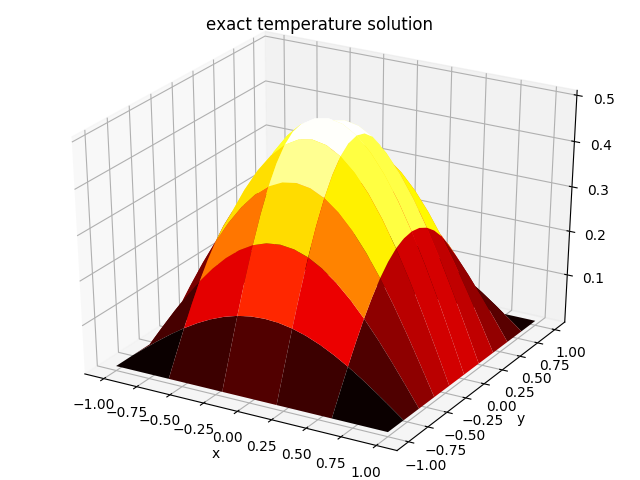
\includegraphics[scale=1]{fig/figure_1.png}
\caption{Surface plot}
\label{fig72}
\end{figure}


\begin{figure}[H]
\centering
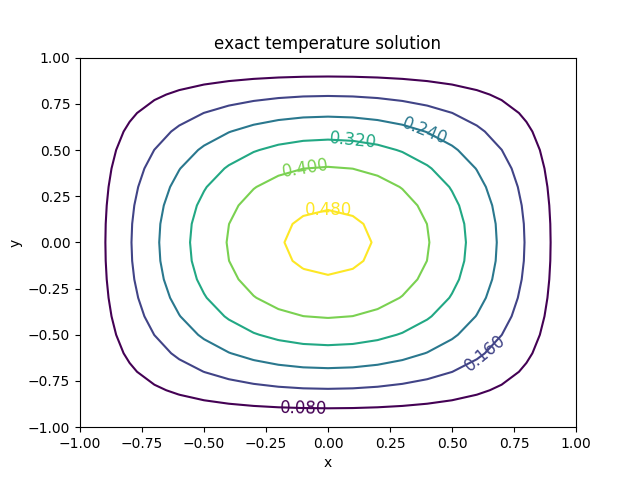
\includegraphics[scale=1]{fig/figure_2.png}
\caption{Contour plot}
\label{fig73}
\end{figure}





\newpage
\subsubsection{Python script}
\label{py3}
\begin{lstlisting}[language=python]
from pylab import *
from mpl_toolkits.mplot3d import Axes3D

# x in units of a, y in units of b, temp. T in units of q'''a^2/k.

fig = figure()
ax = Axes3D(fig)             # create 3D axes
x = np.arange(-1, 1.01, 0.1)
y = np.arange(-1, 1.01, 0.1)
x, y = np.meshgrid(x, y)
z = 0.5 * np.cos(np.pi*x/2) * np.cos(np.pi*y/2)
ax.plot_surface(x, y, z, rstride=2, cstride=4, cmap=cm.hot)
xlabel('x')
ylabel('y')
title('exact temperature solution')

show()

CS = contour(x, y, z)
clabel(CS, inline=0, fontsize=12)
title('exact temperature solution')
xlabel('x')
ylabel('y')
show()

# PS: import * is not recommended (cf import of numpy as np included in the background, confusing) I left it because it works.
\end{lstlisting}
\newpage
